%% State Space Modelling of Dynamic Systems
%% Lecture 1: Introduction to State-Space Models
\def\FileDate{9/9/29}
\def\FileVersion{1.1}
% ----------------------------------------------------------------
% Notes pages *********************************************************
% ----------------------------------------------------------------
\section*{Introduction to State Space}

\begin{slide}\label{slides:l13s1}
\heading{Introduction to State Space}
\begin{itemize}
	\item \emph{Classical control system theory} is based on the Transfer Function model.
	\item Can only be used for systems that are defined by LTI differential equations. 
	\item \emph{Modern control systems theory} is based on a time-domain description of systems.
	\item Convenient matrix form makes the model attractive for simulation, analysis and design using packages like Matlab.
	\item All classical control methods seen so far also apply to state-space models.
\end{itemize}
\end{slide}

Classical control system theory is based on the Transfer Function (TF) model. This applies only to those dynamic systems which can be described by linear time-invariant (LTI) differential equations. TF models are usually applied to Single Input Single Output (SISO) systems. Since the TF is expressed in terms of the Laplace Transform variable, $s$, analysis and design is mostly carried out in the $s$-domain or the frequency domain ($s=j\omega$).

Modern control systems theory is based on a time domain description of a system in terms of a set of first order coupled differential equations in the so-called \emph{state variables} of the system.

State space models can do anything that classical TF models can do.

In addition state space models have allowed control theory to be extended in various directions as shown in \sref{slides:l13s2}

 
\begin{slide}\label{slides:l13s2}
	\heading{The Advances Enabled by State Space Models}
\begin{enumerate}
\item Handling Multiple Input Multiple Output (MIMO) systems.
\item Extension to linear time-varying systems.
\item Clarification of issues of controllability and observability.
\item Development of powerful compensation methods via state feedback and observers.
\item Development of optimal control theory.
\end{enumerate}
\end{slide}
In this module we will restrict ourselves to the study of mostly to SISO LTI systems, but is important to note the possibility of its extension to more challenging areas.

 
\subsection*{Construction of State Space Models}

The state-space model is a form of system representation that is used
in several engineering disciplines. It is particularly used in control
and in signal processing.

The state-space model is a form of differential equation
representation and it is principally used when an analysis of the
system behaviour is required in terms of time responses. That
stated, it is relatively easy to convert a state-space model into
a transfer function, to allow the frequency response analysis of a
system. It is however not necessary to do this conversion if the
time-response behaviour is all that is required.

The state space model is easily extended to cope with models with more
than one input and more than one output. It also has more favourable
numerical properties that make it more attractive as a representation
for high order systems\footnote{Systems with large numbers of
  derivative terms} than the polynomial representation provided by the
transfer function. State-space models are easily simulated by the
straightforward application of numerical integration.

\sref{slides:l13s1} shows a simple electrical circuit. We shall develop
this circuit into a block diagram and from the block-diagram we shall
develop the state-space model. Later we will generalise this result.

\begin{slide}\label{slides:l13s1}
\heading{Example 1}
\begin{center}
\resizebox{150pt}{!}{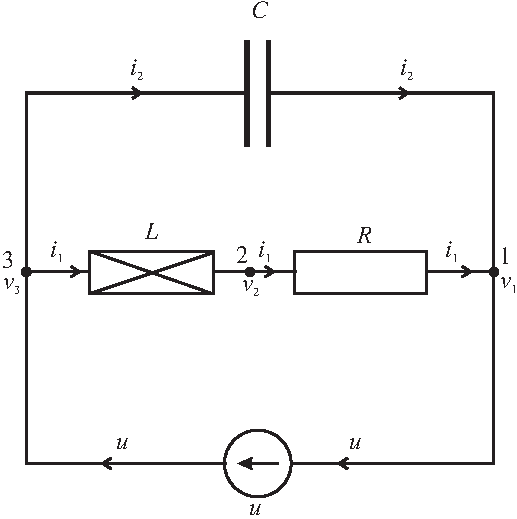
\includegraphics{pictures/circuit.pdf}}
\end{center}
\end{slide}


\ifslidesonly
\begin{slide}\label{opteq:l13e1a}
\heading{Equations}
If we write down the equations for the elements we get:
\begin{eqnarray}
  \frac{dv_{31}}{dt} &=& \frac{1}{C}\ i_2 \label{eq:l13e1}\\
  \frac{di_{i}}{dt} &=& \frac{1}{L}\ v_{32} \label{eq:l13e2}\\
  v_{21} &=& R\ i_1 \label{eq:l13e3}
\end{eqnarray}
The ``compatability'' and ``continuity'' equations are
\begin{eqnarray}
  u &=& i_1 + i_2 \label{eq:l13e4}\\
  v_{31} &=& v_{32} + v_{21} \label{eq:l13e5}
\end{eqnarray}

\endinput
%%% Local Variables: 
%%% mode: latex
%%% TeX-master: "notes"
%%% End: 

\end{slide}
\fiIf we write down the equations for the elements we get:
\begin{eqnarray}
  \frac{dv_{31}}{dt} &=& \frac{1}{C}\ i_2 \label{eq:l13e1}\\
  \frac{di_{i}}{dt} &=& \frac{1}{L}\ v_{32} \label{eq:l13e2}\\
  v_{21} &=& R\ i_1 \label{eq:l13e3}
\end{eqnarray}
The ``compatability'' and ``continuity'' equations are
\begin{eqnarray}
  u &=& i_1 + i_2 \label{eq:l13e4}\\
  v_{31} &=& v_{32} + v_{21} \label{eq:l13e5}
\end{eqnarray}

\endinput
%%% Local Variables: 
%%% mode: latex
%%% TeX-master: "notes"
%%% End: 



Since the system ``source'' is $u$, we can construct the block diagram
systematically by tracing the equations through from the source. We
also introduce the additional constraint that we would like the derivative terms
$dv_{31}/dt$ and $di_1/dt$ to
appear as inputs to integrator blocks whose outputs are therefore
\ifslidesonly
\begin{slide}\label{opteq:l13e1b}
\heading{Equations (continued)}
Integrator equations:
\begin{eqnarray}
  v_{31} = \int \frac{dv_{31}}{dt} dt \label{eq:l13e6}\\
  i_{1} = \int \frac{i_{1}}{dt} dt \label{eq:l13e7}
\end{eqnarray}

\endinput
%%% Local Variables: 
%%% mode: latex
%%% TeX-master: "notes"
%%% End: 

\end{slide}
\fi\begin{eqnarray}
  v_{31} = \int \frac{dv_{31}}{dt} dt \label{eq:l13e6}\\
  i_{1} = \int \frac{i_{1}}{dt} dt \label{eq:l13e7}
\end{eqnarray}

\endinput
%%% Local Variables: 
%%% mode: latex
%%% TeX-master: "notes"
%%% End: 

The other
components of equations (\ref{eq:l13e1}) to (\ref{eq:l13e3}) appear as
gain blocks and (\ref{eq:l13e4}) and (\ref{eq:l13e5}) appear as summing
junctions.  With these constraints, the resulting block diagram is
that shown in \sref{slides:l13s2}.

We can model these equations in \Matlab{}/\Simulink{}\footnote{Note
  that in \Simulink{} triangular blocks are used for gains and that the transfer function
  block $1/s$ represents the integral operator $\int$. The small
  elliptical blocks represent input and output ports.} as shown in \sref{slides:l13s1a}.
\begin{slide}\label{slides:l13s1a}
\heading{Modelled Equations}
\resizebox{300pt}{!}{\rotatebox{90}{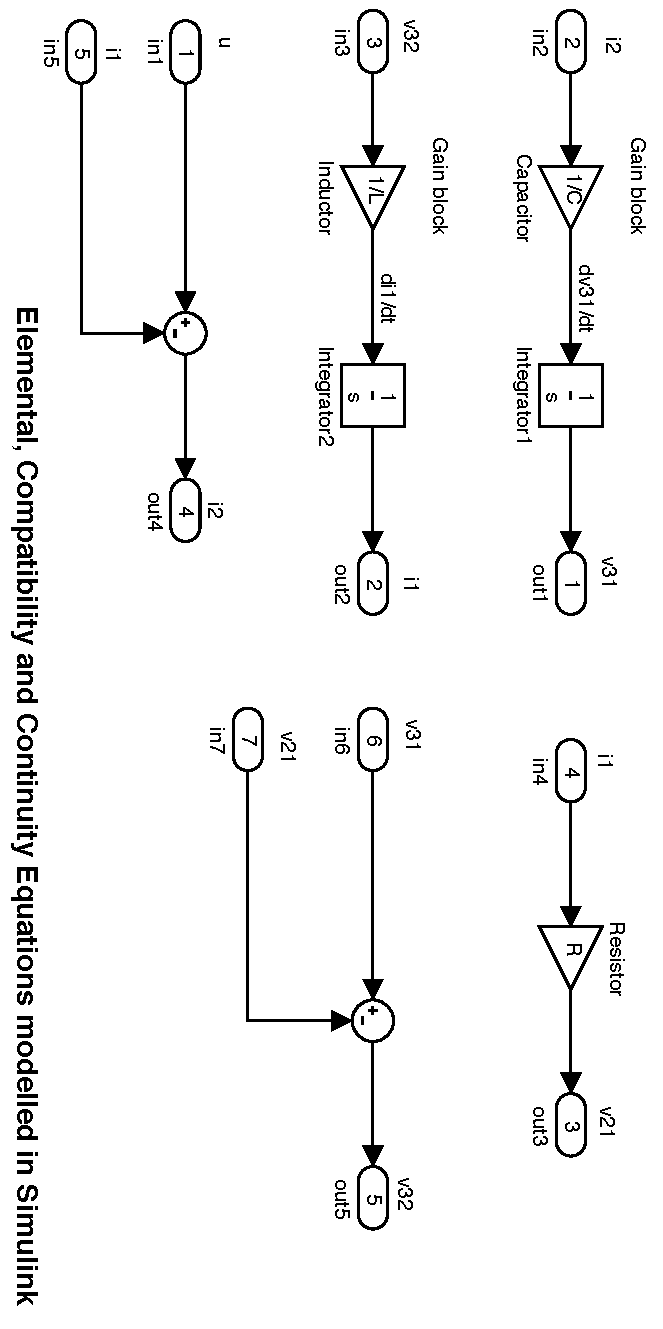
\includegraphics{pictures/blocks.pdf}}}
\end{slide}
Combining these blocks such that the input is $u$ and the output is
the current flowing through the inductance $i_1$\footnote{We could have used any signal as an output as we shall
  see later.} we obtain the block diagram shown in \sref{slides:l13s2}.
\begin{slide}\label{slides:l13s2}
\heading{Example as a Block Diagram}
\resizebox{300pt}{!}{\rotatebox{90}{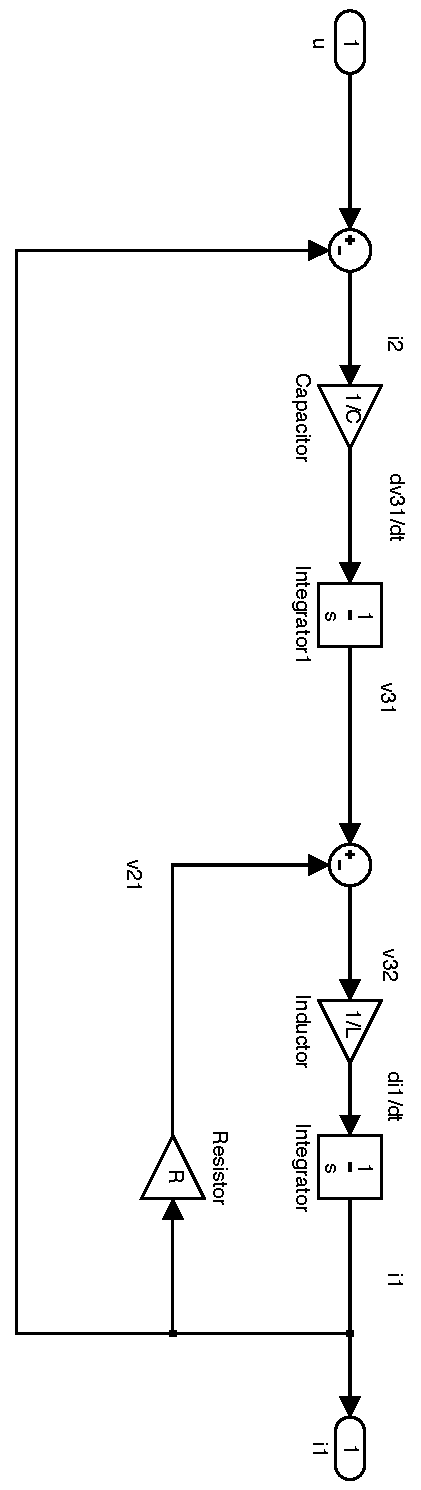
\includegraphics{pictures/blockdiag.pdf}}}
\end{slide}

Having constructed a block diagram that allows us the visualize
the structure of the differential equations, we now go on to
create the state-space model of the system. To do this we first
identify the ``\emph{state-variables}'' which are (in this case)
the physical quantities that are changing with time, i.e. the
voltage across the capacitor $v_{31}$ and the current through the
inductor $i_1$\footnote{A state variable that can be related to a
physical quantity is called a ``\emph{physical state
variable}.''}. The derivatives of these state variables become the
left-hand-side of the ``\emph{state equations}''. These equations
have apparently already been written down as (\ref{eq:l13e1}) and
(\ref{eq:l13e2}), but we impose an additional condition that the
state equations can only involve the state-variables, their
derivatives and the system input. Thus we have to trace the path
back through the block diagram from the inputs to the integrator
blocks to the (nearest) state variable(s). The result is
\ifslidesonly
shown in \sref{slide:ss1}
\begin{slide}\label{slide:ss1}
\heading{State Equations for the Example}
Given the transformation $\mathbf{T}^{-1}\mathbf{AT}=\mathbf{\Lambda}$:
\begin{eqnarray*}
	\mathbf{A}t & = & (\mathbf{T\Lambda T}^{-1}) t \\
	\mathbf{A}^nt^n & = & (\mathbf{T\Lambda T}^{-1})(\mathbf{T\Lambda T}^{-1})\ldots(\mathbf{T\Lambda T}^{-1})t^n \\
	                & = & \mathbf{T\Lambda T}^{-1}\mathbf{T\Lambda T}^{-1}\ldots\mathbf{T\Lambda T}^{-1}t^n \\
	\mathbf{A}^nt^n & = & \mathbf{T\Lambda}\mathbf{I}\mathbf{\Lambda I}\ldots\mathbf{I\Lambda T}^{-1}t^n \\
	\               & = & \mathbf{T\Lambda}^n\mathbf{T}^{-1}t^n \\
\end{eqnarray*}
\endinput

%%% Local Variables: 
%%% mode: latex
%%% TeX-master: "notes"
%%% End:
\end{slide}
\fiGiven the transformation $\mathbf{T}^{-1}\mathbf{AT}=\mathbf{\Lambda}$:
\begin{eqnarray*}
	\mathbf{A}t & = & (\mathbf{T\Lambda T}^{-1}) t \\
	\mathbf{A}^nt^n & = & (\mathbf{T\Lambda T}^{-1})(\mathbf{T\Lambda T}^{-1})\ldots(\mathbf{T\Lambda T}^{-1})t^n \\
	                & = & \mathbf{T\Lambda T}^{-1}\mathbf{T\Lambda T}^{-1}\ldots\mathbf{T\Lambda T}^{-1}t^n \\
	\mathbf{A}^nt^n & = & \mathbf{T\Lambda}\mathbf{I}\mathbf{\Lambda I}\ldots\mathbf{I\Lambda T}^{-1}t^n \\
	\               & = & \mathbf{T\Lambda}^n\mathbf{T}^{-1}t^n \\
\end{eqnarray*}
\endinput

%%% Local Variables: 
%%% mode: latex
%%% TeX-master: "notes"
%%% End:

Equations (\ref{eq:l13e8}) and (\ref{eq:l13e9}) together form a pair
of simultaneous equations (they must both be satisfied by the
dynamic response of the circuit voltages and currents to the
input) and they may therefore be written in vector
form\footnote{You should expand this matrix equation
(\ref{eq:l13e8}) out to verify that it is equivalent to
(\ref{eq:l13e6}) and (\ref{eq:l13e7}).}:
\begin{equation}\label{eq:l13e10}
The matrix function becomes:
\begin{eqnarray*}
	f(\mathbf{A}t) & = & f_0\mathbf{TIT}^{-1} + f_1\mathbf{T\Lambda T}^{-1}t + f_2\mathbf{T\Lambda}^2\mathbf{T}^{-1}t^2 + \cdots + f_n\mathbf{T\Lambda}^n\mathbf{T}^{-1}t^n + \cdots \\
	f(\mathbf{A}t) & = & \mathbf{T}\left(f_0\mathbf{I} + f_1\mathbf{\Lambda}t + f_2\mathbf{\Lambda}^2t^2 + \cdots + f_n\mathbf{\Lambda}^nt^n + \cdots \right)\mathbf{T}^{-1}\\
	               & = & \mathbf{T}f(\mathbf{\Lambda}t)\mathbf{T}^{-1}
\end{eqnarray*}
 
The term inside the brackets on the rhs is a diagonal matrix and the $i^\mathrm{th}$ diagonal element is:
\[
f_0+f_1\lambda_it + f_2\lambda_i^2t^2 + \cdots + f_n\lambda_i^nt^ + \cdots
\]
From the Taylor series this must be $f(\lambda_i t)$:
\[
f(\mathbf{A} t)=\mathbf{T} f(\mathbf{\Lambda} t) \mathbf{T}^{-1}
\]   
where $f(\mathbf{\Lambda} t)=\mathrm{diag}\left(f(\lambda_i t)\right)$.

\endinput

%%% Local Variables: 
%%% mode: latex
%%% TeX-master: "notes"
%%% End:
\end{equation}
\ifslidesonly
\begin{slide}
\heading{State equations in vector form}
\begin{displaymath}
The matrix function becomes:
\begin{eqnarray*}
	f(\mathbf{A}t) & = & f_0\mathbf{TIT}^{-1} + f_1\mathbf{T\Lambda T}^{-1}t + f_2\mathbf{T\Lambda}^2\mathbf{T}^{-1}t^2 + \cdots + f_n\mathbf{T\Lambda}^n\mathbf{T}^{-1}t^n + \cdots \\
	f(\mathbf{A}t) & = & \mathbf{T}\left(f_0\mathbf{I} + f_1\mathbf{\Lambda}t + f_2\mathbf{\Lambda}^2t^2 + \cdots + f_n\mathbf{\Lambda}^nt^n + \cdots \right)\mathbf{T}^{-1}\\
	               & = & \mathbf{T}f(\mathbf{\Lambda}t)\mathbf{T}^{-1}
\end{eqnarray*}
 
The term inside the brackets on the rhs is a diagonal matrix and the $i^\mathrm{th}$ diagonal element is:
\[
f_0+f_1\lambda_it + f_2\lambda_i^2t^2 + \cdots + f_n\lambda_i^nt^ + \cdots
\]
From the Taylor series this must be $f(\lambda_i t)$:
\[
f(\mathbf{A} t)=\mathbf{T} f(\mathbf{\Lambda} t) \mathbf{T}^{-1}
\]   
where $f(\mathbf{\Lambda} t)=\mathrm{diag}\left(f(\lambda_i t)\right)$.

\endinput

%%% Local Variables: 
%%% mode: latex
%%% TeX-master: "notes"
%%% End:
\end{displaymath}
The vector $[v_{31}, i_{1}]^T$ is called the ``\emph{state
vector}.'' Its elements are state variables.
\endinput
%%% Local Variables: 
%%% mode: latex
%%% TeX-master: "notes"
%%% End: 

\end{slide}
\fi
The vector $[v_{31}, i_{1}]^T$ is called the ``\emph{state
vector}.'' Its elements are state variables.
\endinput
%%% Local Variables: 
%%% mode: latex
%%% TeX-master: "notes"
%%% End: 
\footnote{The matrix
operator $[]^T$ is the ``transpose'' operator. In this case it
converts the row vector shown into the column vector actually used
in the state equations. When applied to a matrix, the rows of the
matrix become the columns of the transposed matrix. We shall use
the transpose operator in the discussion of state equations to
avoid messy attempts to write column vectors in the body of a
sentence!}

We can generalize this result by defining general state variables
$x_1=v_{31}$ and $x_2=i_1$. Using the notational shorthand
$\dot{x}=dx/dt$ we then get:
\begin{equation}\label{eq:l13e11}
  \left[\begin{array}{c}
    \dot{x_1} \\
    \dot{x_2} \\
    \end{array}\right]=\left[\begin{array}{cc}
      0 & -1/C \\
      1/L & -R/L \\
    \end{array}\right]\left[\begin{array}{c}
      x_1 \\
      x_2 \\
    \end{array}\right]+\left[\begin{array}{c}
      1/C \\
      0 \\
    \end{array}\right]\ u
\end{equation}
\ifslidesonly
\begin{slide}
\heading{Generalising the Equations}
We can generalize the result by defining general state variables
$x_1=v_{31}$ and $x_2=i_1$. Using the notational shorthand
$\dot{x}=dx/dt$ we then get:
\begin{displaymath}
  \left[\begin{array}{c}
    \dot{x_1} \\
    \dot{x_2} \\
    \end{array}\right]=\left[\begin{array}{cc}
      0 & -1/C \\
      1/L & -R/L \\
    \end{array}\right]\left[\begin{array}{c}
      x_1 \\
      x_2 \\
    \end{array}\right]+\left[\begin{array}{c}
      1/C \\
      0 \\
    \end{array}\right]\ u
\end{displaymath}
\end{slide}
\fi

\subsection*{General State Space Models of Dynamic Systems}

An $n^\mathrm{th}$ order dynamic system can be described by an $n^\mathrm{th}$ order differential equation in one dependent variable, $y(t)$, and an input forcing function, $u(t)$, with time, $t$, as the independent variable.

\begin{equation}
\frac{d^ny}{dt^n}=f\left(\frac{d^{n-1}y}{dt^{n-1}}, \frac{d^{n-2}y}{dt^{n-2}}, \ldots, \frac{dx_2}{dt}, \frac{dy}{dt}, y, u(t), t \right) \label{eq:l13e12}
\end{equation}
\ifslidesonly
\begin{slide}
	\heading{General State Space Models (1)}
	\begin{equation}
	\frac{d^ny}{dt^n}=f\left(\frac{d^{n-1}y}{dt^{n-1}}, \frac{d^{n-2}y}{dt^{n-2}}, \ldots, \frac{dx_2}{dt}, \frac{dy}{dt}, y, u(t), t \right) \nonumber
	\end{equation}
\end{slide}
\fi
Alternatively, in a state space model extra variables, called \textbf{states}, are introduced to create an equivalent description, but this time involving only 1st order differential equations.

\begin{eqnarray}
	x_1 & = & y \label{eq:l13e13a}\\
	\frac{dx_1}{dt} & = & \frac{dy}{dt} = x_2  \label{eq:l13e13b} \\
    \frac{dx_2}{dt} & = & \frac{d^2y}{dt^2} = x_3   \\
	 \vdots      \nonumber \\
	\frac{dx_{n-2}}{dt} & = & \frac{d^{n-2}y}{dt^{n-2}} = x_{n-1}   \\
	\frac{dx_{n-1}}{dt} & = & \frac{d^{n-1}y}{dt^{n-1}} = x_n   \\
    \frac{dx_n}{dt} &=& \frac{d^{n}y}{dt^{n}} =  f\left(x_n, x_{n-1}, \ldots, x_3, x_2, x_1, u(t), t \right) \label{eq:l13e13c}
\end{eqnarray}
\ifslidesonly
\begin{slide}
	\heading{General State Space Models (2)}
	\begin{eqnarray}
		x_1 & = & y \\
		\frac{dx_1}{dt} & = & \frac{dy}{dt} = x_2  \\
	    \frac{dx_2}{dt} & = & \frac{d^2y}{dt^2} = x_3   \\
		 \vdots      \nonumber \\
		\frac{dx_{n-2}}{dt} & = & \frac{d^{n-2}y}{dt^{n-2}} = x_{n-1}   \\
		\frac{dx_{n-1}}{dt} & = & \frac{d^{n-1}y}{dt^{n-1}} = x_n   \\
	    \frac{dx_n}{dt} &=& \frac{d^{n}y}{dt^{n}} =  f\left(x_n, x_{n-1}, \ldots, x_3, x_2, x_1, u(t), t \right) 
	\end{eqnarray}
\end{slide}
\fi
An nth order system gives rise to a state space model consisting of n coupled 1st order differential equations (the \emph{state equations} (\ref{eq:l13e13b})--(\ref{eq:l13e13c})) in terms of $n$ state variables and the input forcing function(s) . In addition there are the \emph{output equations} (\ref{eq:l13e13a}) expressing other variables, or outputs, of interest, also in terms of the states and inputs.

You should note that the formulation used in the differential equation (\ref{eq:l13e12}) and its equivalent state equations (\ref{eq:l13e13a})--(\ref{eq:l13e13c}) is completely general and makes no assumptions about the nature of $f$. In fact the only condition, is that it represents a lumped parameter system rather than a distributed parameter system. The need to solve such equations by simulation is the basis of the integral models we introduced in Lecture 2.
 
\subsubsection*{Example 2}

Derive a state space model for the system described by the differential equation:
 
$$\frac{d^2y}{dt^2}+3\frac{dy}{dt}+2y=u(t)$$
\ifslidesonly
\begin{slide}
	\heading{Example 2}
	
	Derive a state space model for the system described by the differential equation:

	$$\frac{d^2y}{dt^2}+3\frac{dy}{dt}+2y=u(t)$$
\end{slide}
\fi
Introducing state variables $x_1=y$ and $x_2=dy/dt$ then the state equations are:
$$\frac{dx_1}{dt}=\frac{dy}{dt}=x_2$$
$$\frac{dx_2}{dt}=\frac{d^2y}{dt^2}=-2x_1 - 3x_2 + u$$
and the output equation is:
$$y=x_1.$$
 
\begin{slide}
\heading{Physical states}
The states are often chosen to have a direct physical significance such as:

\begin{itemize}
	\item \emph{Electrical Systems} -- the charge or voltage on a capacitor or the current in an inductor.
    \item \emph{Mechanical Systems} -- the force in springs or the velocity of mass or angular velocity of moments of inertia.
    \item \emph{Aerospace Systems} -- forward velocity, thrust, pitch and pitch rate, yaw and yaw rate, position and velocity of control surfaces.
    \item \emph{Chemical Process Plant} -- chemical composition, levels, temperatures, pressures and flows.
\end{itemize}
\end{slide}

\begin{slide}
	\heading{Example 3}
	Derive the state equations for the Sprig-Mass-Damper system shown in the figure.
	\begin{center}
		\resizebox{100pt}{!}{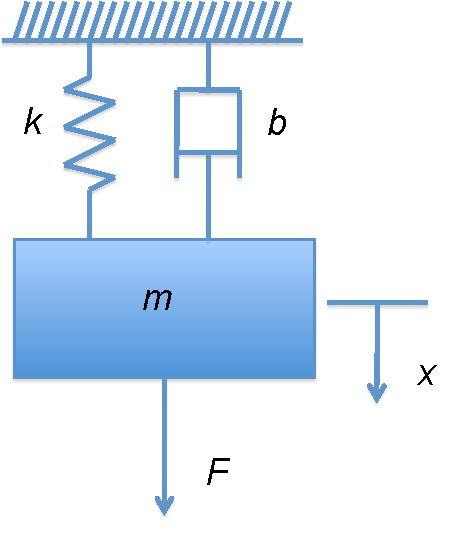
\includegraphics{pictures/smd.pdf}}
	\end{center}
	(See lecture 2)
\end{slide}

For this system, summing the forces in the direction $x$ we have

$$F = m\frac{d^2x}{dt^2} + b\frac{dx}{dt} + kx$$

If we chose the position of the mass $x$ and it's velocity $dx/dt$ to be the states, and let the force $F$ be the system input, then $x_1 = x$, $x_2 = dx/dt$ and $u=F$ and the state equations are:

\begin{eqnarray*}
	\frac{dx_1}{dt} & = & x_2 \\
	\frac{dx_2}{dt} & = & -\frac{k}{m} x_1 -\frac{b}{m} x_2 + \frac{1}{m} u
\end{eqnarray*}

You should construct the Simulink model represented by these equations and compare the results with those shown in Lecture 2.

\subsection*{The nature of the states}

\begin{itemize}
	\item The state equations can be solved uniquely when the input functions are given together with the initial values of all the states.
	\item The solutions for the states are substituted into the output equations to obtain the solutions for the other variables in the system.
	\item In the above examples the states are physical quantities associated with energy storage in the system. The energy stored in a inductor is $E_L=Li_L^2/2$, and the energy stored in a capacitor is $E_C=CV_C^2/2$. 
	\item Similarly for mechanical systems the velocity of a mass relates to its kinetic energy and the force in a spring relates to its elastic potential energy.
	\item The states encode the configuration of the system, or its whole past history.
	\item The choice of states is not unique, but they must be chosen such that the configuration of the system can be unambiguously and completely determined from them.
\end{itemize}
\ifslidesonly
\begin{slide}
	\heading{State Properties}
	\begin{itemize}
	\item The state equations can be solved for a given input function and initial conditions.
	\item Other variables in the system can be determined from the state solutions and the output equations.
	\item Physical states are associated with energy storage.
	\item The states encode a system's whole past history.
	\item The choice of states is not unique.
\end{itemize}
\end{slide}
\fi
 
\subsection*{State Space Models for Linear Systems}

Linear systems are the most important ones for control system analysis and design as the best methods and techniques apply to these.

Non-linear systems are often approximated about a suitable operating point by the nearest equivalent linear system allowing linear techniques to be used in the design of a suitable controller.

In the case of linear systems, each state equation expresses the derivative of one of the states as a linear function of the states and inputs. The output equations also express the output variables linearly. As a consequence the natural mathematical notation to use is that of vectors and matrices.
Thus state, input and output variables are grouped in column vectors and are multiplied by matrices in the state and output equations.

For linear time varying systems, the matrices have elements which are functions of time, but for time invariant systems all the matrices are constant.
\ifslidesonly
\begin{slide}
	\heading{State Space Models for Linear Systems}
	\begin{itemize}
	 \item Linear systems most important for control systems analysis and design.
	 \item Best control methods and techniques apply to linear systems.
	 \item Nonlinear systems can often be \emph{linearized} around a given operating point allowing linear methods to be used.
	 \item Linear models can be modelled with matrix equations with makes them attractive to tools like Matlab.
	 \item Linear time-varying systems have matrix elements which are functions of time.
	 \item Linear time invariant systems have constant matrix elements.
  \end{itemize}
\end{slide}
\fi

\subsubsection*{A vector/matrix notation}

In general, we will have $n$ state variables and $q$ system
inputs. In such a case we can write down a matrix state
equation as developed in \sref{slides:l13s3} and \sref{slides:l13s4}.
\begin{slide}\label{slides:l13s3}
\heading{Matrix State Equation (1)} Let us define a general
$n$-dimensional state vector
\[\mathbf{x} = \left[x_1,\ x_2,\ \ldots, x_n\right]^T\] Its
derivative is
\[\frac{d\mathbf{x}}{dt} = \left[\frac{dx_1}{dt},\ \frac{dx_2}{dt},\
\ldots,\
\frac{dx_n}{dt}\right]^T\] or more compactly
\[\dot{\mathbf{x}}=\left[\dot{x_1},\ \dot{x_2},\ \ldots,\
\dot{x_n}\right]^T.\]

There may be any number of inputs to a system, so we also assume a
general vector of $q$ inputs
\[\mathbf{u}=\left[u_1,\ u_2,\ \ldots,\ u_q\right]^T\]
\end{slide}

\begin{slide}\label{slides:l13s4}
\heading{Matrix State Equation (2)}
\[
\dot{\mathbf{x}}=\left[\begin{array}{cccc}
  a_{11} & a_{12} & \cdots & a_{1n} \\
  a_{21} & a_{22} & \cdots & a_{2n} \\
  \vdots & \vdots & \ddots & \vdots \\
  a_{n1} & a_{n2} & \cdots & a_{nn}
\end{array}\right]\ \mathbf{x} + \left[\begin{array}{cccc}
  b_{11} & b_{12} & \cdots & b_{1q} \\
  b_{21} & b_{22} & \cdots & b_{2q} \\
  \vdots & \vdots & \ddots & \vdots \\
  b_{n1} & b_{n2} & \cdots & b_{nq}
\end{array}\right]\ \mathbf{u} \\
\]
or more succinctly
\[
\dot{\mathbf{x}}=\mathbf{A}\mathbf{x}+\mathbf{B}\mathbf{u}
\]
Where $\mathbf{A}$ is the $n\times n$ ``\emph{system matrix}'' and
$\mathbf{B}$ is the $n\times q$ ``\emph{input matrix}''.
\end{slide}


The state equations allow us to describe the internal behaviour of
the system when subjected to stimuli from the inputs. In 
example 1, we need nothing more if we wish to describe the way that
the capacitor voltage $v_{31}$ and inductor current $i_1$ change
with time under the influence of the input current $u$. However,
if we wish to describe the behaviour of the other variables in the
circuit we need to complete the state space model with a set of
``\emph{output equations}.''

Let us consider every possible output. From the block diagram, we
see that, in terms of the state variables and the system input
\begin{eqnarray}
\label{eq:l13y1} v_{31}&=&1\times v_{31} \\
i_1 & = & 1\times i_1 \\
v_{32} &=& 1\times v_{31} - R \times i_1 \\ 
v_{21} & = & R \times i_1 \\ 
\label{eq:l13yn} i_2 & = & u - 1\times i_1.
\end{eqnarray}
\ifslidesonly
\begin{slide}
\heading{Output Equations}
For illustration purposes we write an ``output equation'' for every
possible signal.
\begin{eqnarray*}
v_{31}&=&1\times v_{31} \\
i_1 & = & 1\times i_1 \\ 
v_{32} &=& 1\times v_{31} - R \times i_1 \\ 
v_{21} & = & R \times i_1\\ 
i_2 & = & u - 1\times i_1.
\end{eqnarray*}
\end{slide}
\fi
Arranging these equations in vector form we have:
\begin{equation}
\left[\begin{array}{c}
  v_{31} \\
  i_1 \\
  v_{32} \\
  v_{21} \\
  i_2
\end{array}\right] = \left[\begin{array}{cc}
  1 & 0 \\
  0 & 1 \\
  1 & -R \\
  0 & R \\
  0 & -1
\end{array}\right]\ \left[\begin{array}{c}
  v_{31} \\
  i_1
\end{array}\right]+\left[\begin{array}{c}
  0 \\
  0 \\
  0 \\
  0 \\
  1
\end{array}\right] u
\end{equation}
\ifslidesonly
\begin{slide}
\heading{Vectorised form...}
Arranging the output equations in vector form we have:
\begin{displaymath}
\left[\begin{array}{c}
  v_{31} \\
  i_1 \\
  v_{32} \\
  v_{21} \\
  i_2
\end{array}\right] = \left[\begin{array}{cc}
  1 & 0 \\
  0 & 1 \\
  1 & -R \\
  0 & R \\
  0 & -1
\end{array}\right]\ \left[\begin{array}{c}
  v_{31} \\
  i_1
\end{array}\right]+\left[\begin{array}{c}
  0 \\
  0 \\
  0 \\
  0 \\
  1
\end{array}\right] u
\end{displaymath}
\end{slide}
\fi
In general, we can describe a system with $r$ inputs in terms of
the generic output variables $y_1, y_2,\ldots,\ y_r$ as shown in
\sref{slides:l13s5} and \sref{slides:l13s6}.
\begin{slide}\label{slides:l13s5}
\heading{General Output Equation (1)} Let us define a general
output vector
\[\mathbf{y} = \left[y_1,\ y_2,\ \ldots, y_r\right]^T\]

Given that some of the inputs to the system may be directly
connected to the output, the input vector may also appear in the
output general equation.
\end{slide}
\begin{slide}\label{slides:l13s6}
\heading{General Output Equation (2)}
\[
\mathbf{y}=\left[\begin{array}{cccc}
  c_{11} & c_{12} & \cdots & c_{1n} \\
  c_{21} & c_{22} & \cdots & c_{2n} \\
  \vdots & \vdots & \vdots & \vdots \\
  c_{r1} & c_{r2} & \cdots & c_{rn}
\end{array}\right]\ \mathbf{x} + \left[\begin{array}{cccc}
  d_{11} & d_{12} & \cdots & d_{1q} \\
  d_{21} & d_{22} & \cdots & d_{2q} \\
  \vdots & \vdots & \vdots & \vdots \\
  d_{r1} & d_{r2} & \cdots & d_{rq}
\end{array}\right]\ \mathbf{u} \\
\]
or more succinctly
\[
\mathbf{y}=\mathbf{C}\mathbf{x}+\mathbf{D}\mathbf{u}
\]
Where $\mathbf{C}$ is the $n\times r$ ``\emph{output matrix}'' and
$\mathbf{D}$ is the $r\times q$ ``\emph{feedforward matrix}''.
\end{slide} This
equation relates the states and inputs to the outputs. There are
no dynamic terms!
\begin{slide}\label{slides:l13s7}
\heading{The State Space Model}
\begin{eqnarray*}
\dot{\mathbf{x}}&=&\mathbf{A}\mathbf{x}+\mathbf{B}\mathbf{u}\\
{y}&=&\mathbf{C}\mathbf{x}+\mathbf{D}\mathbf{u}
\end{eqnarray*}
Can always be developed from a system with physically realizable
states and physical realistic sources. Such a system is called
``\emph{proper}''. If $\mathbf{D}$ is null (matrix of zeros) the
system is called ``\emph{strictly proper}''.
\end{slide}
A block diagram representation of the state space model is shown
in \sref{slides:l13s8}. The block diagram of the circuit, rearranged
to match the general model is shown in \sref{slides:l13s9}.
\begin{slide}\label{slides:l13s8}
\heading{Block Diagram of a State-Space Model}
\resizebox{300pt}{!}{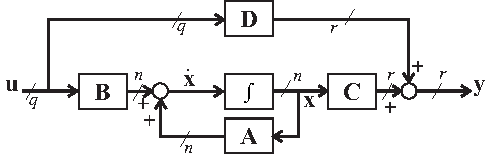
\includegraphics{pictures/ssmodel}}
\end{slide}
\begin{slide}\label{slides:l13s9}
\heading{State Space Model of Example 1}
\resizebox{300pt}{!}{\rotatebox{90}{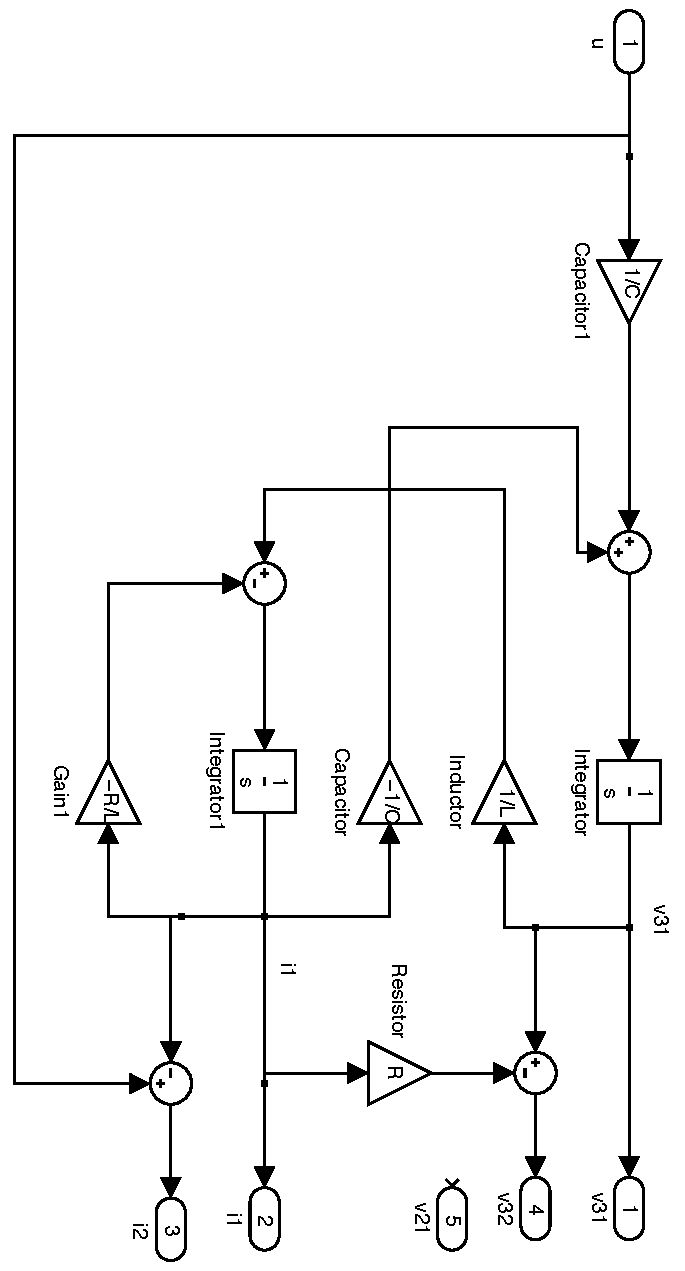
\includegraphics{pictures/statemodel.pdf}}}
\end{slide}

\subsubsection*{Modelling State Space Systems in Matlab}

\begin{slide}
	\heading{Modelling State Space Systems in Matlab}
	For the example above
	\begin{verbatim}
	A = [0 -1/Cap; 1/L -R/L];
	B = [1/Cap; 0];
	C = [1 0; 0 1; 1 -R; 0 R; 0 -1];
	D = [0; 0; 0; 0; 1];
	circ_ss = ss(A, B, C, D, ...
	   'statename',{'v31' 'i1'}, 'inputname', 'u', 'outputname', {'v31' 'i1' 'v32' 'v21' 'i2'});	
	\end{verbatim}
	Once you have the state-space model, all the analysis techniques seen so far are open to you.
\end{slide}


%----------------------------------------------------------------
% The end of slides
% ----------------------------------------------------------------
\endinput

% Local Variables:
% TeX-master: "lecture1"
% End:
